\documentclass[
    draft=false,
    paper=a4,
    fontsize=11pt,
    twoside=false,
    captions=tableheading,
    british, ngerman,
]{scrartcl}

\usepackage{babel}

\usepackage{libertine}
\usepackage{libertinust1math}

\usepackage[utf8]{inputenc}
\usepackage[T1]{fontenc}
\usepackage[final]{microtype}

\usepackage{booktabs}
\usepackage{csquotes}
%\usepackage{minipage}
\usepackage{graphicx}
\usepackage{siunitx}

\usepackage{hyperref}

\setkomafont{captionlabel}{%
    \bfseries
}
\setkomafont{caption}{%
    \bfseries
}
\setcapindent{0em}

\begin{document}

\begin{center}
    \LARGE\textsf{\textbf{Plan für User Study}}
\end{center}

\noindent
Im Rahmen dieser Masterarbeit wird untersucht, ob sich eine digitale, in die Umgebung integrierte 3D-Karte für die Anwendung der Kartenexploration eignet.
Zu diesem Zweck wird das Konzept der Megamap vorgestellt und mittels VR-Technologie prototypisch implementiert.
Zum Testen der Implementierung werden Explorationsaufgaben durchgeführt, die von bereits existierenden Kartenanwendungen inspiriert sind.

Das Ziel dieser Studie ist zu ermitteln, welche Parameterwerte die Megamap für Nutzer \emph{angenehm nutzbar} machen.
Ebenso soll ermittelt werden, ob die Parameterwerte Einfluss auf die \emph{Effektivität} der Nutzer haben.

\section{Setup}
Das Experiment wird (vorraussichtlich) im Laborraum 5230 des MZH an der Uni Bremen durchgeführt.
Als Hardware wird ein Desktop-PC inklusive Monitor (für den Versuchsleiter) sowie ein \emph{HTC Vive} HMD inklusive Lighthouses und Controller eingesetzt.
\autoref{fig:study_design_rework} zeigt eine Skizze der Testsituation.
Der Proband befindet sich in einer virtuellen Nachbildung des Laborraums im Maßstab $1:1$.
Die Ausgangsposition, an die der Nutzer sich zu Beginn stellen soll, ist sowohl in der echten als auch der virtuellen Umgebung mit einem \textbf{X} gekennzeichnet.
Dadurch werden die reale und virtuelle Position synchronisiert.

Dem Probanden wird (je nach Kondition, siehe \autoref{sec:conditions}) die Megamap eines Gebäudestockwerks gezeigt.
Virtuelle Stecknadeln (\emph{Pins}) weisen auf interessante Punkte hin.
Dies sind die Zielobjekte der durchzuführenden Aufgaben (\emph{Tasks}, siehe \autoref{sec:tasks}).
\begin{figure}[p]
    \centering
    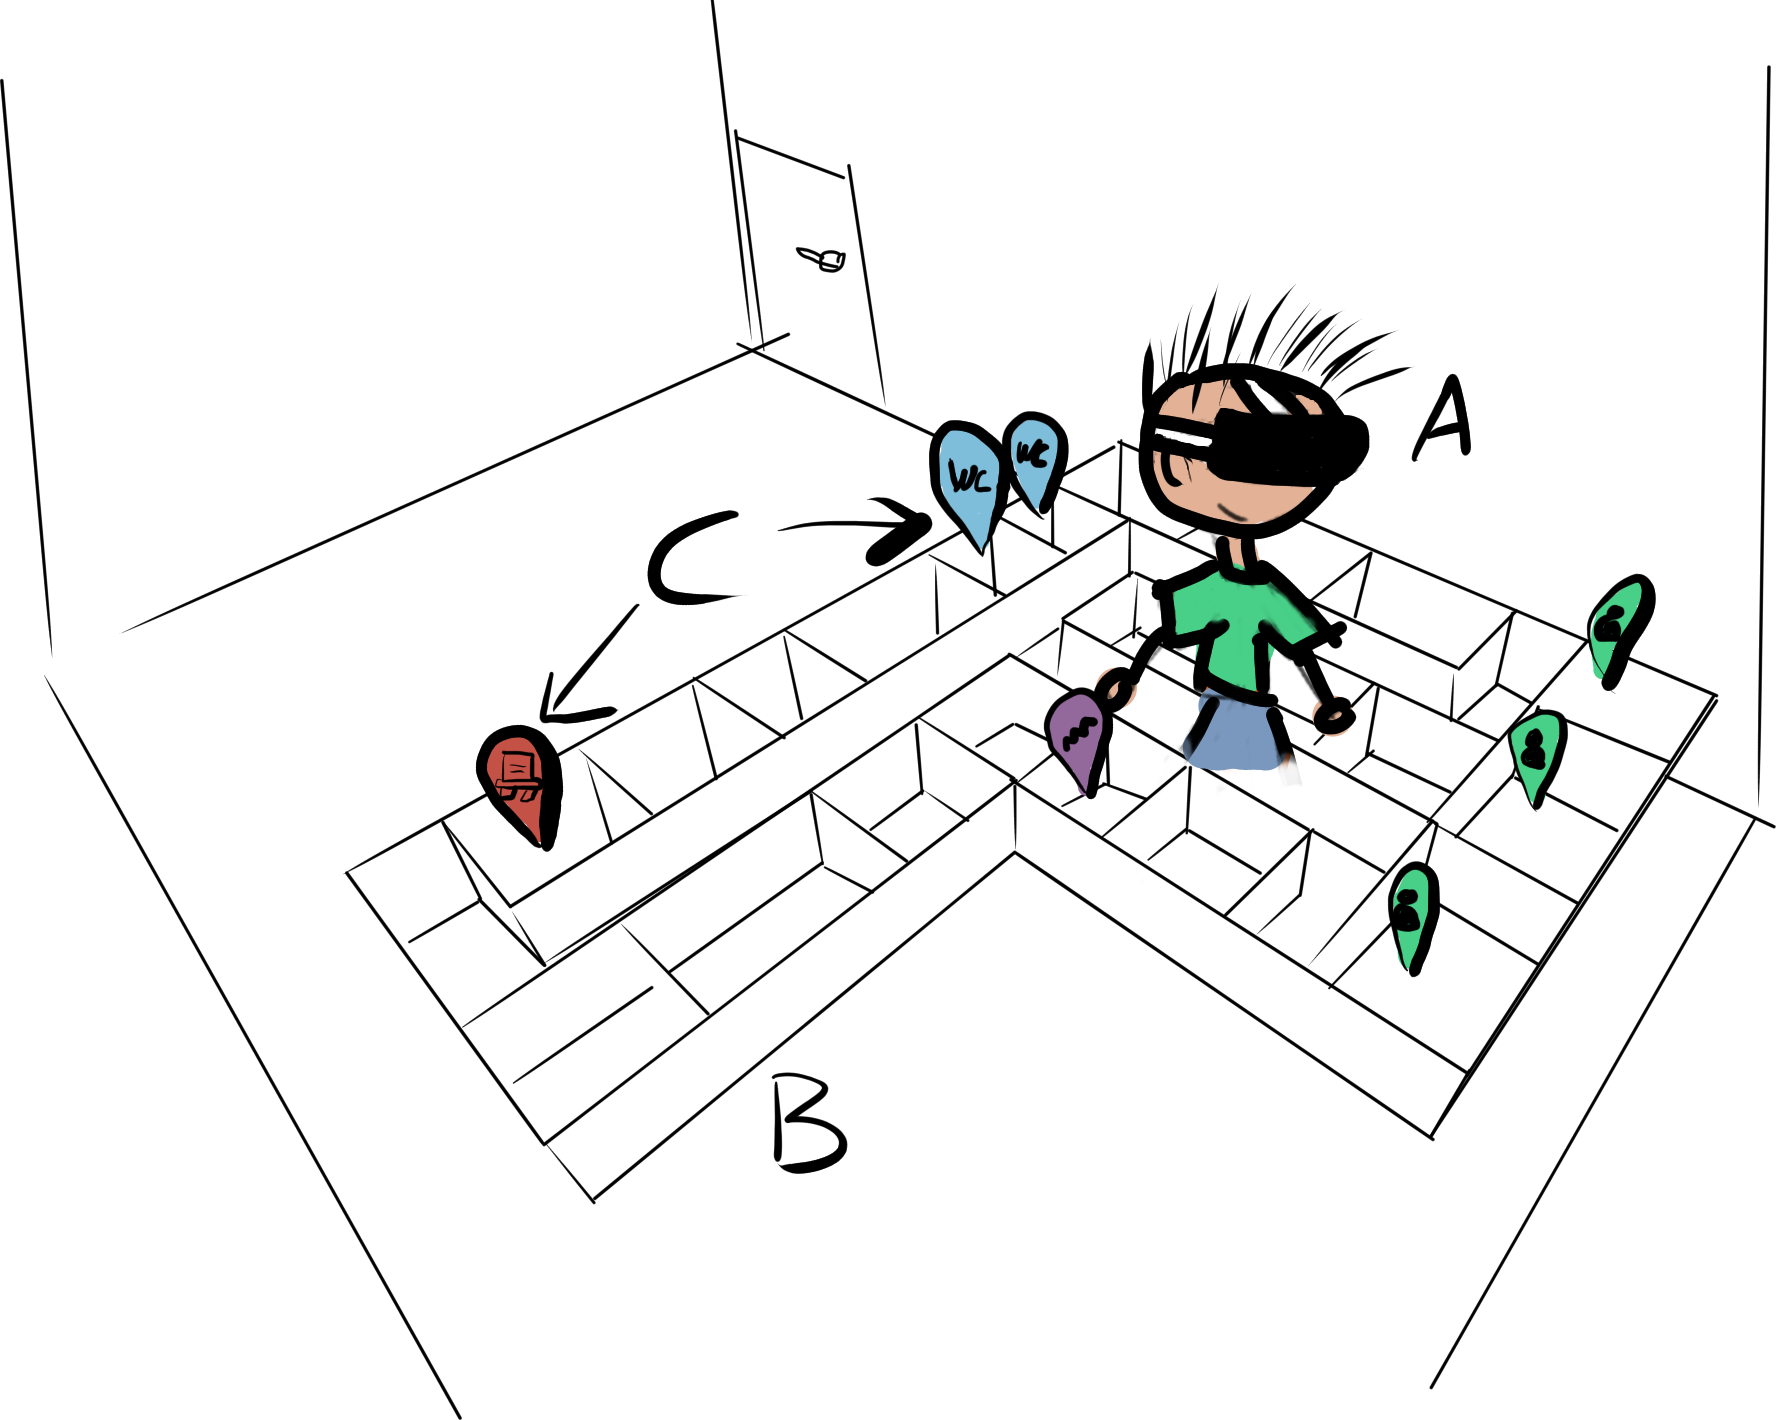
\includegraphics[width=0.9\textwidth]{study_design_setup_reworked}
    \caption{Übersicht des Megamap-Testsetups. %
    \textbf{(A)} Der Nutzer trägt ein \emph{HTC Vive HMD}. %
    Er befindet sich in einer virtuellen Nachbildung des Testlabors. %
    Seine Position im virtuellen Labor entspricht der Position im realen Labor. %
    \textbf{(B)} Um den Nutzer wird die Megamap einer Etage eines imaginären Gebäudes angezeigt. %
    \textbf{(C)} Virtuelle Stecknadeln weisen auf die unterschiedlichen Zielobjekte hin (WC, Drucker, Büro, Treppe).}
    \label{fig:study_design_rework}
\end{figure}

% TODO: Sind 8 Konditionen nicht zu viel?
\section{Konditionen}
\label{sec:conditions}
Ziel dieser Studie ist, die von den Probanden prä\-fe\-rier\-ten Einstellungen der Megamap-Ei\-gen\-schaf\-ten Skalierung\ $S$, Kartenhöhe\ $H$ und Wandhöhe\ $W$ zu ermitteln (siehe \autoref{fig:study_design_parameters}).
\begin{figure}[p]
    \centering
    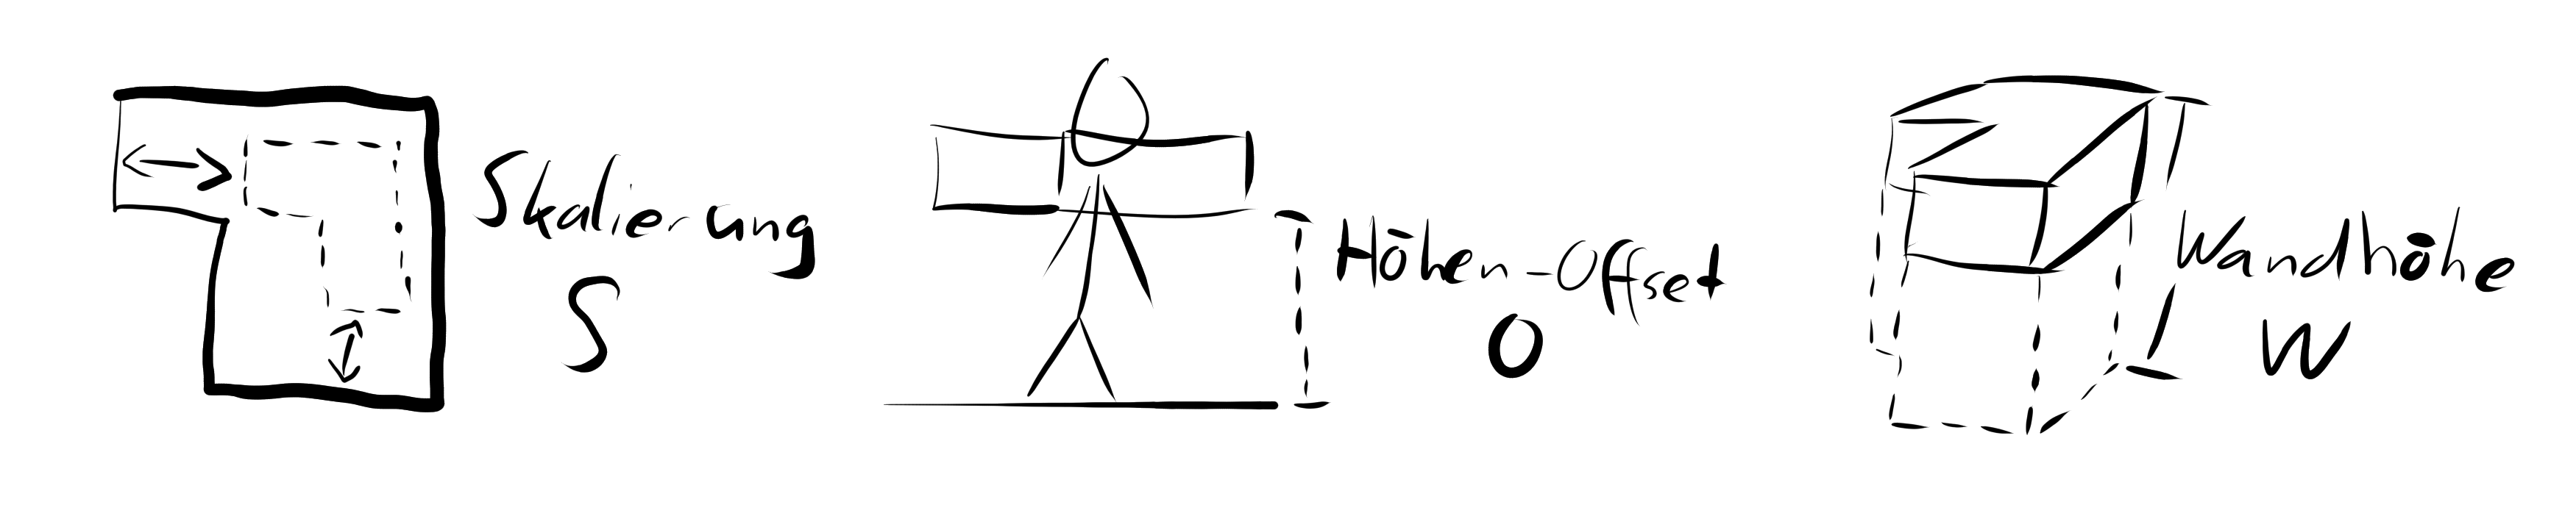
\includegraphics[width=\textwidth]{study_design_parameters}
    \caption{Für die Eigenschaften Skalierung $S$, Kartenhöhe $H$ und Wandhöhe $W$ der Megamap sind die Präferenzen der Nutzer zu ermitteln.}
    \label{fig:study_design_parameters}
\end{figure}
Für die unterschiedlichen Eigenschaften werden jeweils zwei Werte getestet: \emph{niedrig} (\emph{low}/$_l$) und \emph{hoch} (\emph{high}/$_h$).
\autoref{tab:values} gibt die entsprechenden Werte an.
% TODO: Werte aus Unity einsetzen.
\begin{table}[hb]
    \centering
    \caption{Die zu testenden Parameterwerte der Megamap. %
    Vorab durch Versuchsleiter festgelegt.}
    \label{tab:values}
    \begin{tabular}{cccc}
        Wert & $S$ [Verhältnis Karte zu Umgebung] & $H$ [in \si{\meter}] & $W$ [???] \\\toprule
        \emph{low} & 1 : ??? & & \\\midrule
        \emph{high} & 1 : ??? & & \\\bottomrule
    \end{tabular}
\end{table}

Insgesamt ergeben sich also acht Konditionen $K_1 \dots K_8$:
\begin{align*}
    &K_1: \lbrack S_l, O_l, W_l \rbrack, && K_5: \lbrack S_h, O_l, W_l \rbrack\\
    &K_2: \lbrack S_l, O_h, W_l \rbrack, && K_6: \lbrack S_h, O_h, W_l \rbrack,\\
    &K_3: \lbrack S_l, O_l, W_h \rbrack, && K_7: \lbrack S_h, O_l, W_h \rbrack,\\
    &K_4: \lbrack S_l, O_h, W_h \rbrack, && K_8: \lbrack S_h, O_h, W_h \rbrack
\end{align*}
Jeder Proband durchläuft alle acht Konditionen.
Für jede Kondition werden drei Aufgaben durchgeführt (siehe \autoref{sec:tasks}).
Weiterhin wird für jede Kondition eine andere Megamap verwendet.
Alle Megamaps haben die gleiche Anzahl an Räumen.
Außerdem findet sich in jeder Karte die gleiche Anzahl an virtuellen Stecknadeln.
Die Anordnung (Position) der Räume sowie der virtuellen Stecknadeln variiert jedoch.
So soll ein Lerneffekt zwischen den einzelnen Konditionen vermieden werden.

\section{Aufgaben}
\label{sec:tasks}
Für jede Kondition führen Probanden drei Aufgaben durch.
Hierfür müssen die Probanden auf der Megamap Zielobjekte finden, die durch virtuelle Stecknadeln makiert sind (siehe \autoref{fig:study_design_rework}).
Die Zielobjekte lassen sich anhand der Farbe und Icons der Stecknadeln unterscheiden.
Die Aufgabe für die Probanden besteht darin, sich in der virtuellen Umgebung zu den gesuchten Zielobjekten bzw. deren Stecknadeln zu bewegen.
Die Probanden \enquote{berühren} dann mit dem Vive-Controller die Stecknadel und drücken den Trigger, wodurch sich ein Informationsfeld zu dem Ort öffnet.
Ebenfalls wird ein Button zum Auswählen des Zielobjekts dargestellt, welcher ebenfalls durch den Trigger des Controllers betätigt werden kann.
Das Auswählen dient der Zeitmessung.
% TODO: Mehr auf Zeitmessung eingehen.

Die drei Aufgaben laufen immer nach dem gleichen Schema ab:
\begin{enumerate}
    \item Der Proband sucht nach dem Büro einer benannten Person (\enquote{Finde auf der Megamap das Büro von \dots.}). %
    Der Name der Person ist durch Auswahl der Büro-Stecknadel sichtbar. %
    Bei dieser Aufgabe wird ein spezifisches Zielobjekt gesucht.
    \item Der Proband sucht ein beliebiges Zielobjekt aus mehreren möglichen aus (\enquote{Finde auf der Megamap \textbf{einen} Drucker}). %
    Dies ist eine offene Suche.
    \item Der Proband sucht ein spezielles Zielobjekt auf mehreren möglichen aus (\enquote{Finde auf der Megamap \textbf{das nächste} WC}). %
    Dies ist eine semi-offene Suche.
\end{enumerate}
Nachdem das Zielobjekt ausgewählt ist (siehe oben), wird die Megamap ausgeblendet, sodass nur die virtuelle Umgebung sichtbar ist.
Die Probanden sollen mit dem Vive-Controller nun in die Richtung zeigen, in der sich das Zielobjekt in ihrer Umgebung befindet.
Ein ausgehender Strahl vom Controller assistiert bei der Visualisierung der Richtung.
Die Probanden bestätigen die Richtung durch Betätigen eines Knopfs am Controller.
Durch diese Zeige-Aufgaben soll ermittelt werden, ob die unterschiedlichen Konditionen Einfluss auf das räumliche Verständnis der Prbanden haben, unabhängig von deren Präferenzen.
Nach der Zeige-Aufgabe folgt die nächste Such-Aufgabe bzw. die nächste Kondition.

Da alle drei Aufgaben mit der selben Megamap durchgeführt werden, laufen diese immer in der oben gennanten Reihenfolge ab, um so den Lerneffekt in die gemessenen Zeiten miteinbeziehen zu können und die Vergleichbarkeit der Konditionen zu erhalten.

Als Zielobjekte für die Aufgaben 2 und 3 stehen WCs, Drucker, und Treppen zur Auswahl.
Das Zielobjekt \enquote{Büro} wird nur in der ersten Aufgabe verwendet, da hier nach spezifischen Personen.

Zusammengefasst absolviert ein Proband demnach 24 Aufgaben (\emph{Tasks}) $T$:
\begin{gather*}
    K_1: T_{1, 1}, T_{1, 2}, T_{1, 3} \\
    K_2: T_{2, 1}, T_{2, 2}, T_{2, 3} \\
    \vdots \\
    K_8: T_{8, 1}, T_{8, 2}, T_{8, 3}
\end{gather*}

% TODO: Durchführung beschreiben. Tutorial nicht vergessen.
\section{Ablauf}

\end{document}
